\documentclass{article}

\usepackage[portuguese]{babel}

\usepackage{amsmath, amssymb}
\usepackage{graphicx}
\usepackage[colorlinks=true, allcolors=blue]{hyperref}

\usepackage[section]{placeins}

\title{Relatório 03}
\author{Vinícius de Oliveira Peixoto Rodrigues (245294)}
\date{Agosto de 2022}

\begin{document}
\maketitle

\section*{Item (c)}

O analisador léxico serve como um transpilador, convertendo código em uma linguagem arbitrária para código em C. A tabela abaixo lista as substituições mais simples feitas pelo lexer:

\begin{center}
\begin{tabular}{ |c|c|c| }
    \hline
    \textbf{símbolo} & \textbf{tradução em C} & \textbf{observação} \\ \hline
    \texttt{\{...\}} & \texttt{/*...*/} & \\ \hline
    \texttt{mod} & \texttt{\%} & \\ \hline
    \texttt{or} & \texttt{||} & \\ \hline
    \texttt{and} & \texttt{\&\&} & \\ \hline
    \texttt{:=} & \texttt{=} & \\ \hline
    \texttt{<>} & \texttt{==} & \\ \hline
    \texttt{><} & \texttt{!=} & \\ \hline
    \texttt{><} & \texttt{!=} & \\ \hline
    \texttt{><} & \texttt{!=} & \\ \hline
    \texttt{var} &  & ignorado quando em uma linha isolada \\ \hline
    \texttt{bar} &  & ignorado quando em uma linha isolada \\ \hline
    \texttt{.} &  & ignorado \\ \hline
\end{tabular}
\end{center}

Além dessas substituições simples, há duas coisas importantes. A primeira é que o seguinte pattern:

tem a intenção de dar match em expressões da forma
\begin{verbatim}
program <program_name>(<params>);
\end{verbatim}

apesar de consumir agressivamente qualquer linha que comece com

\begin{verbatim}
program[qualquer coisa](
\end{verbatim}

Ao fazer match desse padrão, o programa "abre" a definição de função \texttt{main() \{}, que só é "fechada" depois pela keyword \texttt{end}, que será substituída pela chave de fechamento (\texttt{\}}). Desse modo, o programa inteiro se encontra dentro da \texttt{main()} transpilada.

Outro ponto importante é a declaração de variáveis inteiras, na seguinte forma:

\begin{verbatim}
var
    <varlist> : integer;
\end{verbatim}

onde o lexer descarta (ignora) a keyword \texttt{var} e dá match segundo a regra

\begin{verbatim}
^.*integer;     ShuffleInt();
\end{verbatim}

ou seja, consumindo a nova linha seguinte inteira (por isso o \texttt{\textasciicircum}) desde que ela termine em \texttt{integer}. A função \texttt{ShuffleInt()}, por sua vez, faz o parse da lista de argumentos (basicamente fazendo o prepend da keyword \texttt{int} e copiando caractere por caractere tudo que vem antes de \texttt{: integer;}) (por isso a condição de parada \texttt{yytext[i] != ':'}).

\newpage
\section*{Item (d)}

O programa cria a \textit{start condition} \texttt{Palavra}:

\begin{verbatim}
    %START Palavra
\end{verbatim}

E cria também as labels \texttt{NovaLinha}, \texttt{Espaco} e \texttt{NovaPagina}. Em seguida, sempre que o lexer encontra uma dessas três ocorrências, incrementa o contador adequado. 
Sempre que for encontrado algo que não corresponde a nenhum dentre os três casos \texttt{NovaLinha}, \texttt{Espaco} e \texttt{NovaPagina}, o parser incrementa o contador de palavras e passa para o estado \texttt{Palavra}, onde ele consome caracteres até encontrar \texttt{NovaLinha}, \texttt{Espaco} ou \texttt{NovaPagina}.
Quando isso ocorre, o parser retorna pro estado 0 (inicial) e o ciclo de consumir todos os \texttt{NovaLinha}/\texttt{Espaco}/\texttt{NovaPagina} subsequentes $\rightarrow$ trocar para o estado \texttt{Palavra} e consumir todos os caracteres até o próximo espaço/newline/newpage se repete até ser encontrado o EOF.

\begin{figure}[!ht]
    \begin{center}
        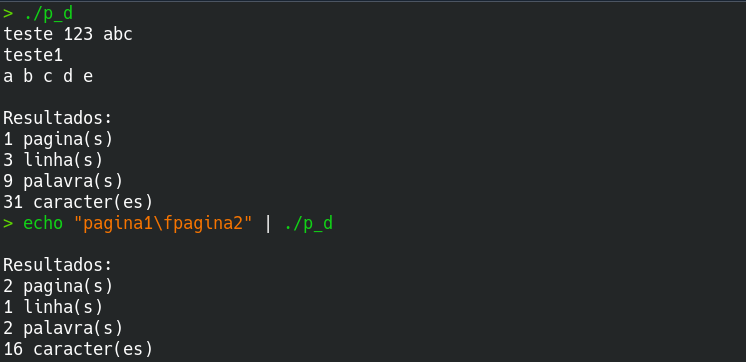
\includegraphics[width=\textwidth]{images/item_d.png}
        \caption{Testes do lexer \texttt{p\_d}}
    \end{center}
\end{figure} 

\newpage
\section*{Item (e)}

O programa dá match em números escritos em formato octal e os imprime em formato decimal, utilizando o \texttt{sscanf()} com o formatador \texttt{"\%o"} para ler o número e guardar na variável \texttt{valor}, e o \texttt{printf("\%d", valor)} para imprimi-lo em decimal.

\begin{figure}[!ht]
    \begin{center}
        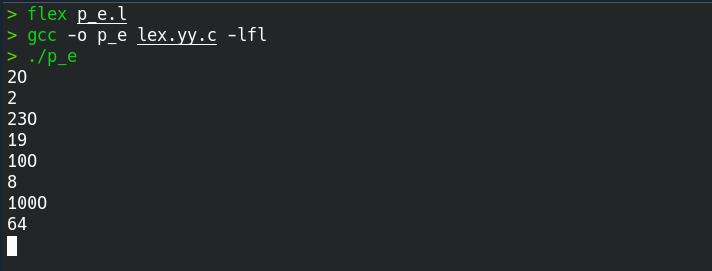
\includegraphics[width=\textwidth]{images/item_e.png}
        \caption{Testes do lexer \texttt{p\_e}}
    \end{center}
\end{figure} 

\section*{Itens (f) e (g)}

Os scripts se encontram em anexo.

\begin{figure}[!ht]
    \begin{center}
        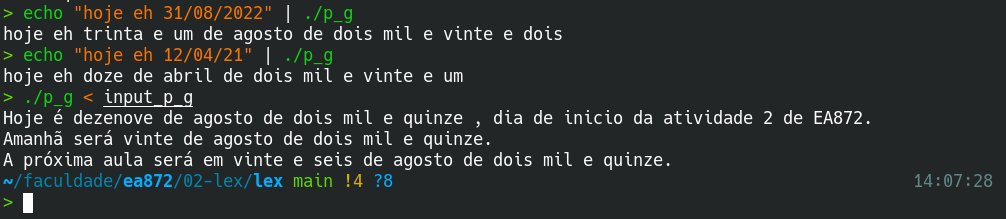
\includegraphics[width=\textwidth]{images/item_g.png}
        \caption{Testes do lexer \texttt{p\_g}}
    \end{center}
\end{figure} 

\end{document}